\providecommand{\main}{../../../..}
\documentclass[\main/dresen_thesis.tex]{subfiles}

\begin{document}
  \label{sec:monolayers:preparation:nanoparticleVariation}
    \begin{figure}[tb]
      \centering
      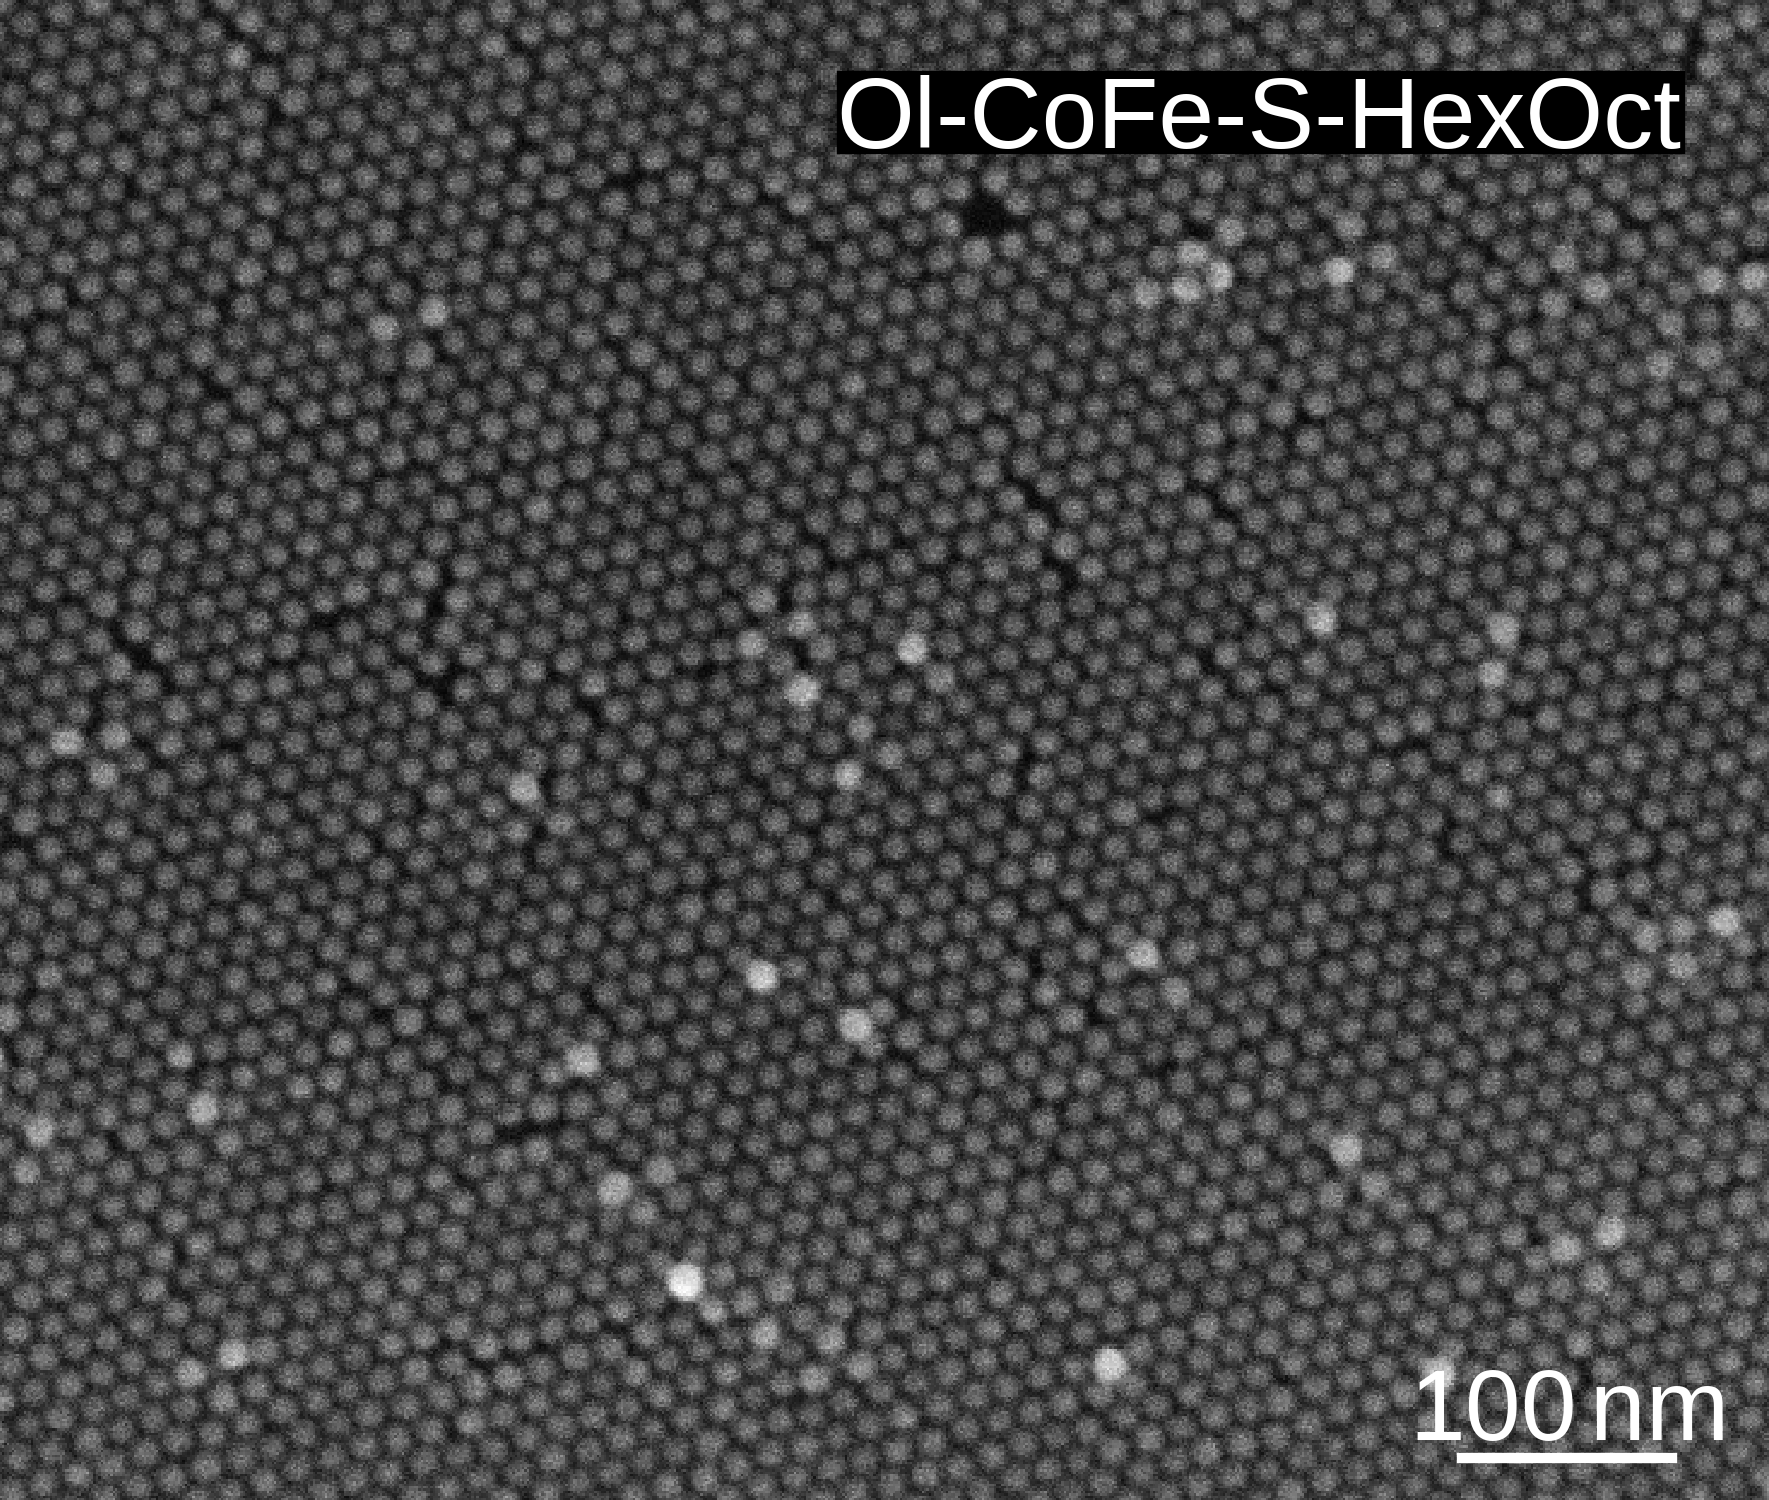
\includegraphics{monolayers_SEM_Ol-CoFe-S-HexOct}
      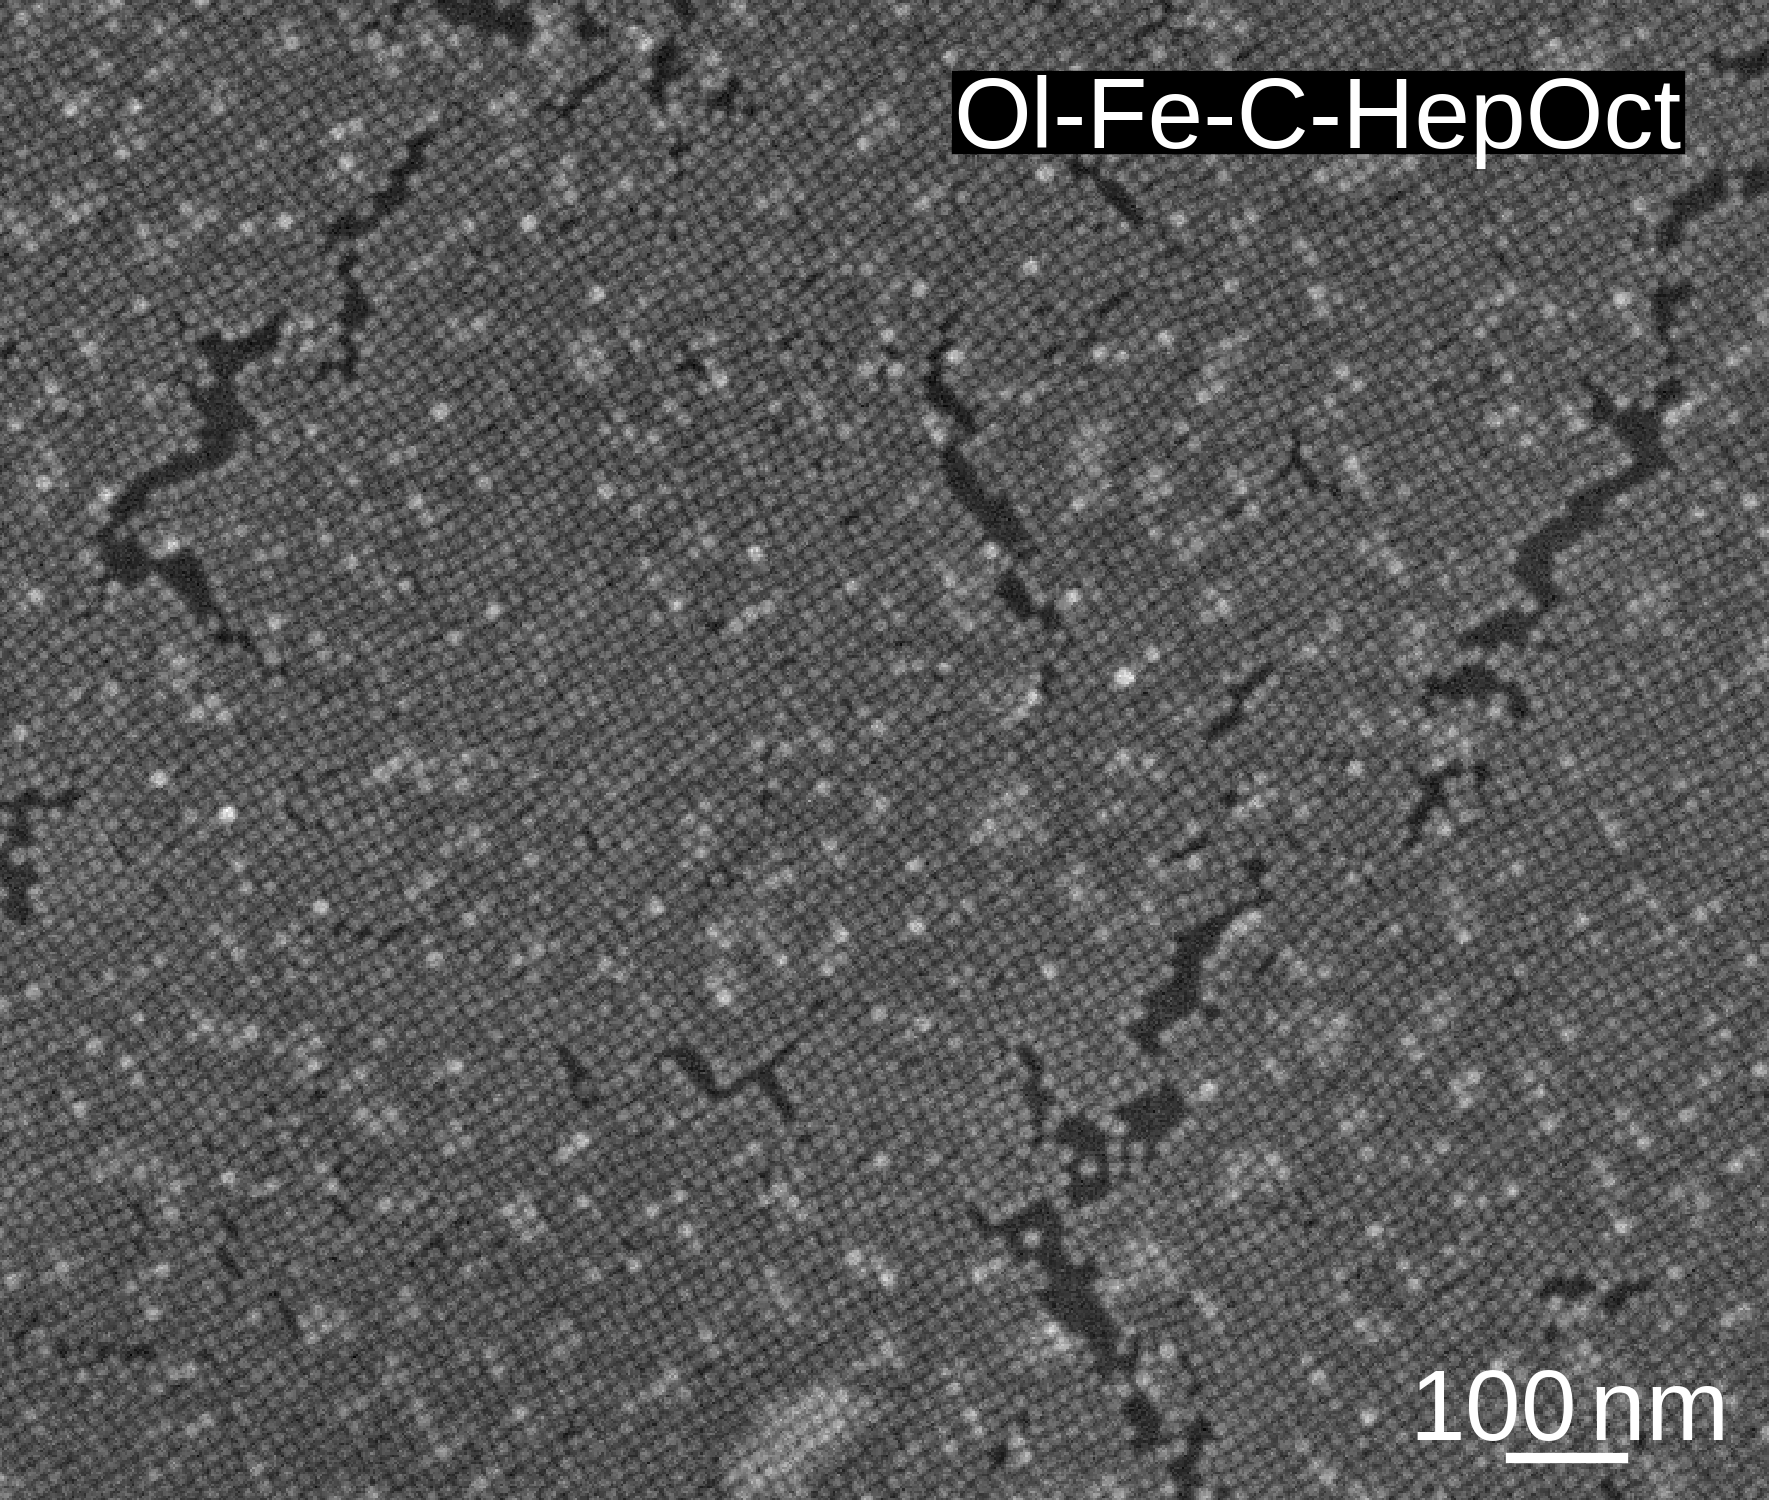
\includegraphics{monolayers_SEM_Ol-Fe-C-HepOct}
      \caption{\label{fig:monolayers:preparation:nanoparticleVariation:spheresIron}Micrographs of cobalt ferrite nanospheres (left) and iron oxide nanocubes (right) deposited as monolayers using octadecene as co-solvent.}
    \end{figure}

    To show that the developed drop casting protocol can be transferred to other nanoparticle batches, it has been applied to dispersions of cobalt ferrite nanospheres and iron oxide nanocubes shown in \reffig{fig:monolayers:preparation:nanoparticleVariation:spheresIron}.
    For the cobalt ferrite nanospheres in Ol-CoFe-S-HexOct and iron oxide nanocubes, hexagonal order and square order is observed, respectively.

    This underlines that the choice of the particle shape determines the relative positioning of the nanoparticles in the monolayer.
    This observation is interesting for an extended study of the dipolar magnetism due to it's directional nature.
    Furthermore, as the order is transferable to other materials such as iron oxide, the relative strength of dipolar interaction and the magnetic anisotropy in the nanoparticle arrays can be tuned.
\end{document}